\documentclass{article}
\usepackage{graphicx}
\usepackage{amsmath}
\usepackage{listings}
\usepackage{caption}
\usepackage[hidelinks]{hyperref}
\setlength{\parindent}{0pt}


\begin{document}
    

\begin{titlepage}
    \vbox{ }
    \vbox{ }
    \begin{center}
        % Set course here
        % TIØ4120 - Operasjonsanalyse, grunnkurs
        % TDT4136 - Introduction to Artificial Intelligence
        
\includegraphics[width=0.40\textwidth]{NTNU_logo.png}\\[1cm]
    \textsc{\Large TIØ4120 - Operasjonsanalyse, grunnkurs}\\[0.5cm]
    \vbox{ }
    
    % Set title here
    { \huge \bfseries Exercise \#1}\\[0.4cm]
    
    \large
    \emph{Author:}\\
    Sondre Pedersen
    \vfill
    
    {\large\today}
\end{center}
\end{titlepage}
    
    \captionsetup[figure]{labelformat=empty}


    \section*{\textbf{Oppgave 1: Grafisk illustrering}}
    \small\textbf{3.1-2 For each of the following constraints, draw a separate graph to show the nonnegative solutions that satisfy this constraint.}
    
    \begin{figure}[ht]
        \centering
        \begin{minipage}{0.3\textwidth}
            \centering
            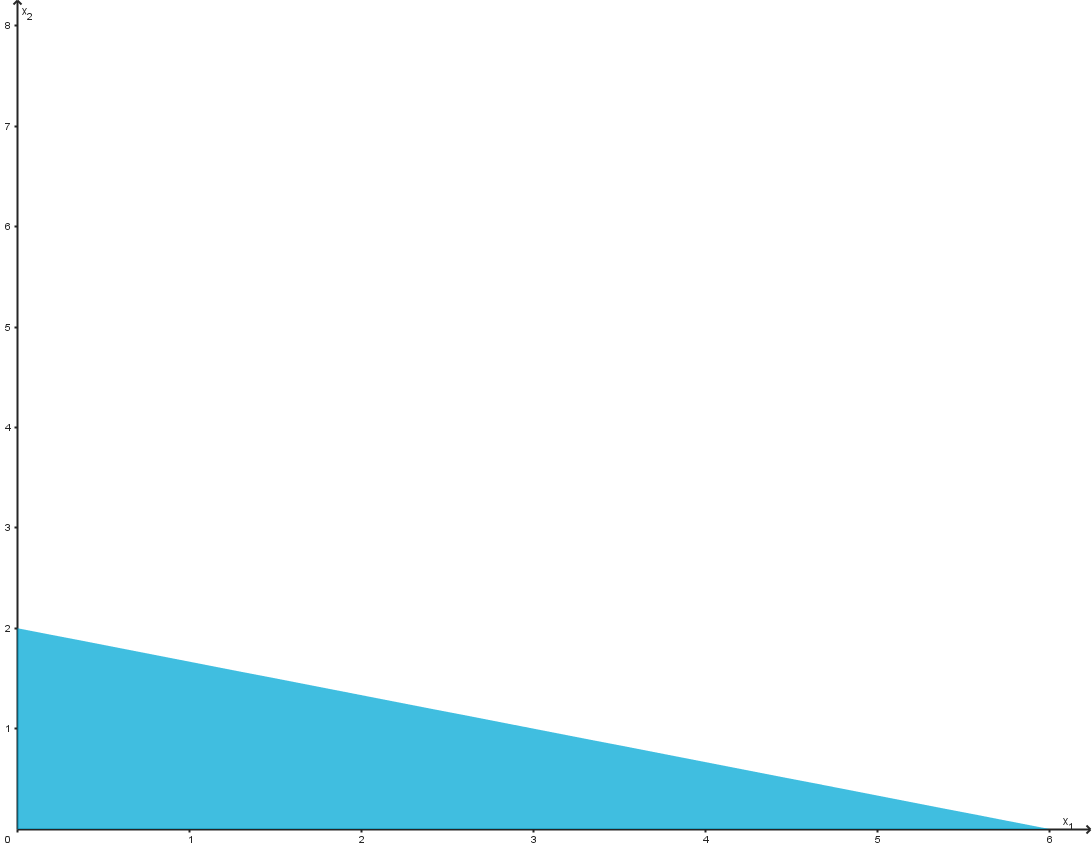
\includegraphics[width=\linewidth]{img/3.1-2a.PNG}
            \caption{a) $x_1 + 3x_2 <= 6$}
        \end{minipage}\hfill
        \begin{minipage}{0.3\textwidth}
            \centering
            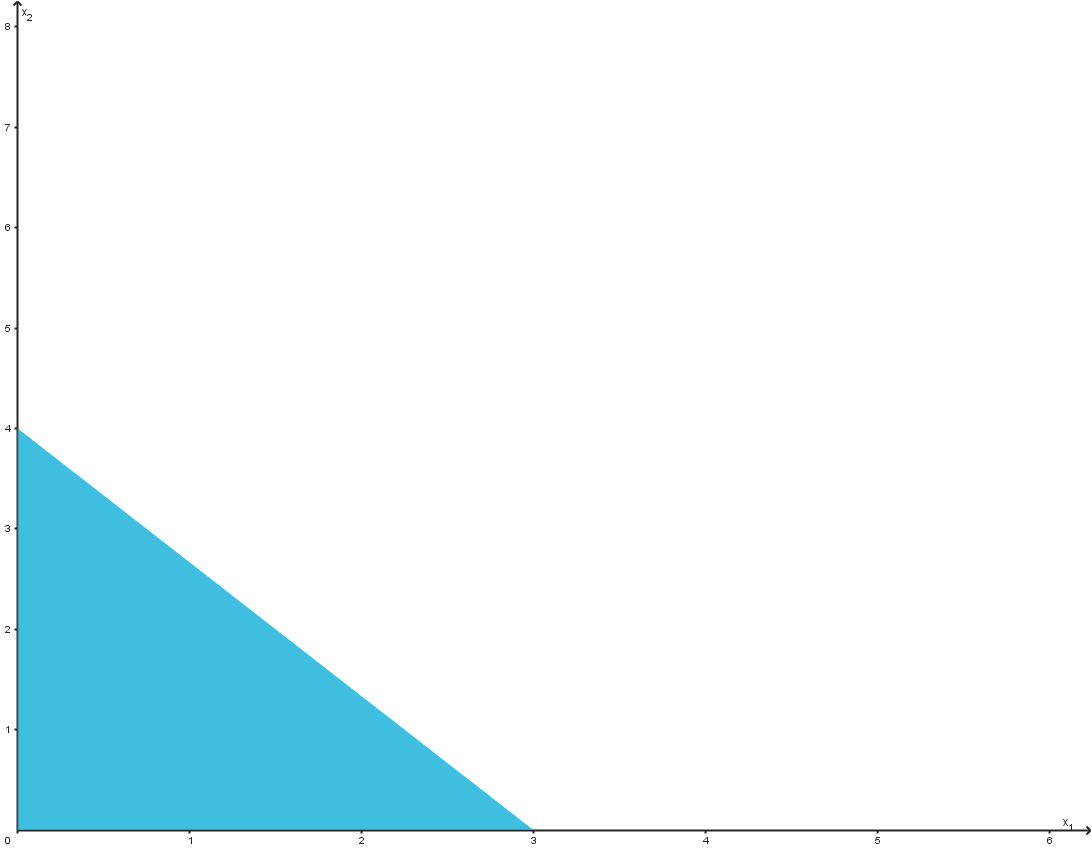
\includegraphics[width=\linewidth]{img/3.1-2b.PNG}
            \caption{b) $4x_1 + 3x_2 <= 12$}
        \end{minipage}\hfill
        \begin{minipage}{0.3\textwidth}
            \centering
            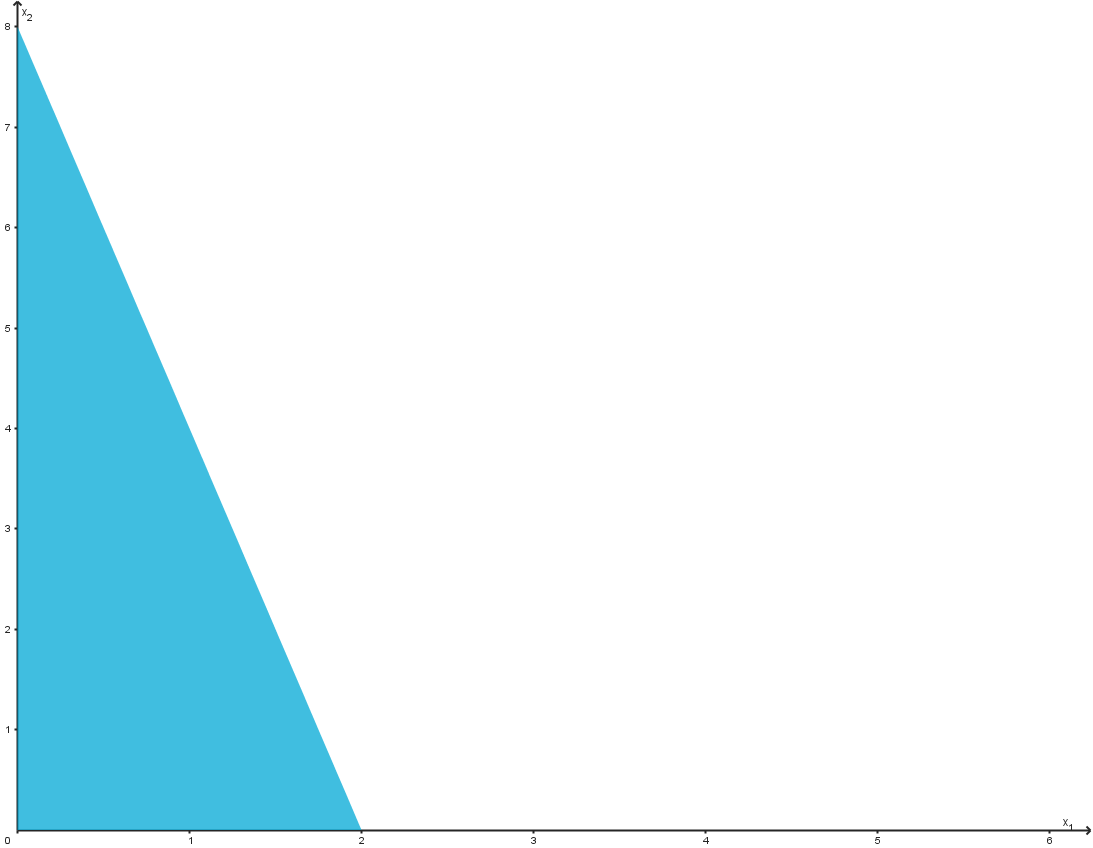
\includegraphics[width=\linewidth]{img/3.1-2c.PNG}
            \caption{c) $4x_1 + x_2 <= 8$}
        \end{minipage}
    \end{figure}
    
    \begin{figure}[ht]
        \centering
        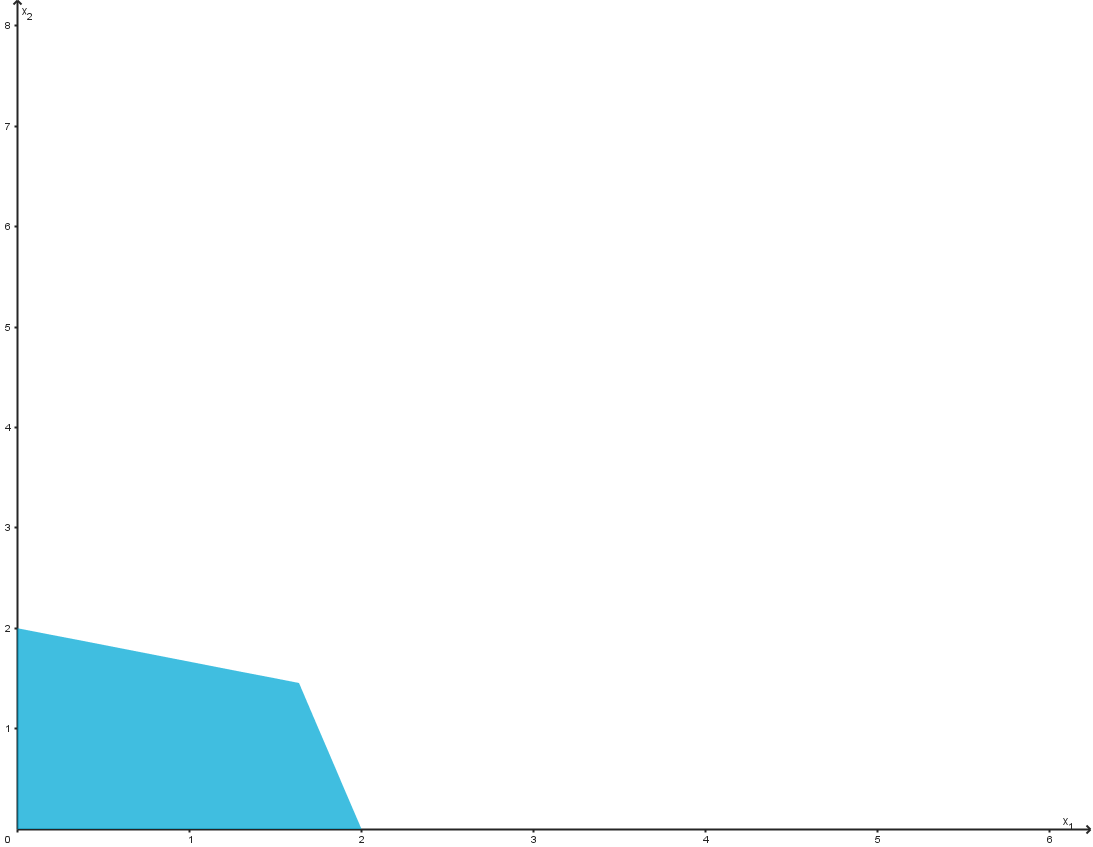
\includegraphics[width=0.5\linewidth]{img/3.1-2d.PNG}
        \caption{d) $a \land b \land c$}
    \end{figure}

    Beklager blanding mellom norsk og engelsk i denne innleveringen. Jeg følger språket brukt i oppgavebeskrivelsen. 
    
    \pagebreak\small\textbf{3.1-3 Consider the following objective function for a linear programming model:} \textit{Maximize Z = $2x_1 + 3x_2, Z_1 = 6, Z_2 = 12, Z_3 = 18$}
    \begin{figure}[ht]
        \centering
        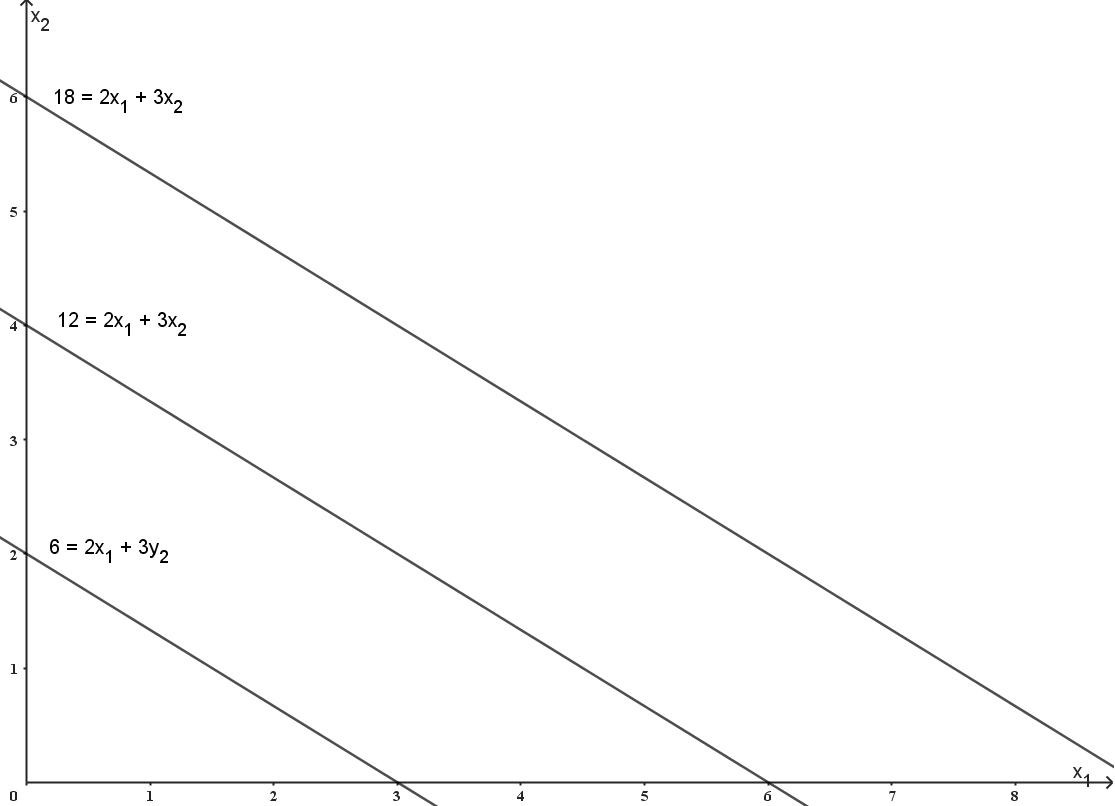
\includegraphics[width=0.8\linewidth]{img/3.1-3a.PNG}
        \caption{a) Objective functions}
    \end{figure}
    
    \small\textbf{b) }
    
    \begin{align*}
        Z_i &= 2x_1 + 3x_2 \\
        \Rightarrow x_2 &= \frac{Z_i}{3} - \frac{2x_1}{3} \\   
        slope &= \frac{dx_2}{dx_1} = -\frac{2}{3}     
    \end{align*}
    
    They have the same slope. From the graph, we can see that the $x_2$ intercept is 2, 4, 6. The interception increases along with Z.
    
    \pagebreak\section*{\textbf{Oppgave 2: Max problem}}
    
    \small\textit{max z = $3x_1 + 6x_2$ når}
    \begin{align*}
        & 3x_1 + 2x_2 <= 18 \\
        & x_1 + x_2 <= 5 \\
        & x_1 <= 4 \\
        & x_2 <= 7 \\
        & \frac{x_2}{x_1} <= \frac{7}{8}\\
        & x_1 >= 0 \\
        & x_2 >= 0
    \end{align*}
    
    \begin{figure}[ht]
        \centering
        \begin{minipage}{0.45\textwidth}
            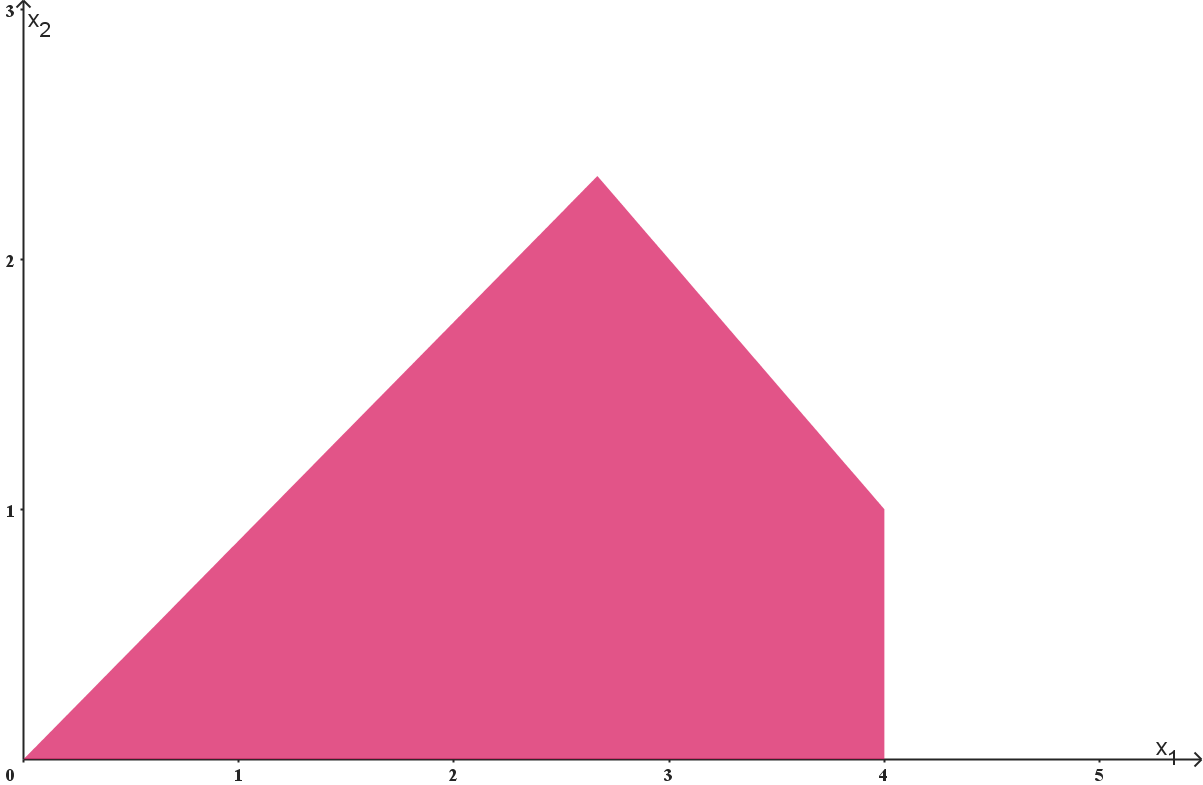
\includegraphics[width=\linewidth]{img/2a.PNG}
            \caption{a) Mulighetsområde}
        \end{minipage}
        \begin{minipage}{0.45\textwidth}
            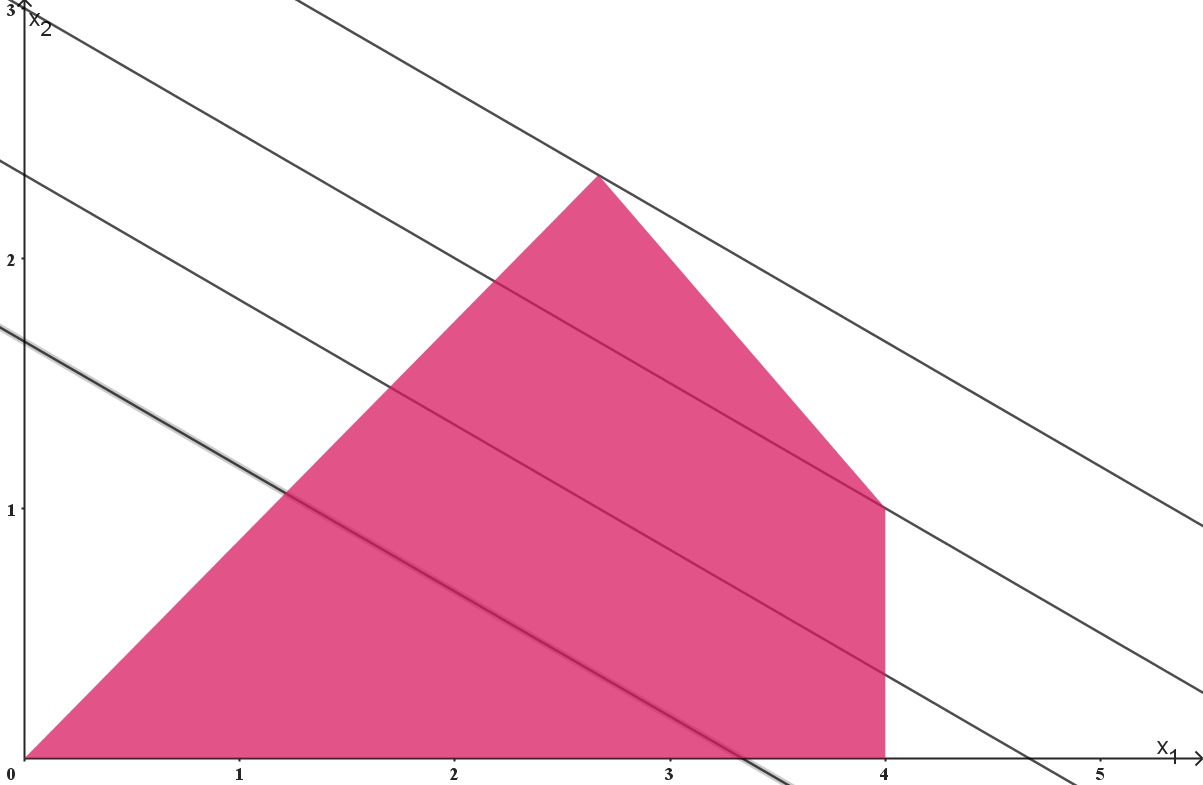
\includegraphics[width=\linewidth]{img/2b.PNG}
            \caption{a) Z = 10, 14, 18, 22}
        \end{minipage}
    \end{figure}
    
    Løser ved å lage en målfunksjon der Z = 10, og øke Z til bare ett punkt på linjen er innenfor Mulighetsområdet.
    
    \small\textbf{b)}
    
    Løsningen er når Z = 22. Løser finner $x_1$ og $x_2$ ved å se at punktet er møtepunktet mellom $x_1 + x_2 = 5$ og $\frac{x_2}{x_1} = \frac{7}{8} \Rightarrow 8x_2 - 7x_1 = 0$. 
    Ved å løse ligningssettet får vi $x_1 = \frac{8}{3}$ og $x_2 = \frac{7}{3} $
    
    \pagebreak\section*{\textbf{Oppgave 3: Excel}}
    \small\textbf{3.5-5 Investment}
    
    LP formulated problem:
    
    min z = $2.5x_1 + 3x_2 + 3.5x_4$ such that
    
    \begin{align}
        & 2x_1 + 1x_2 + 0.5x_3 >= 400 \\
        & 0.5x_1 + 0.5x_2 + x_3 >= 100 \\
        & 1.5x_2 + 2x_3 >= 300
    \end{align}
    
    Where all units are millions of dollars. $x_i$ refer to asset i.
    
    \small\textbf{c), d)}
    
    \begin{figure}[ht]
        \centering
        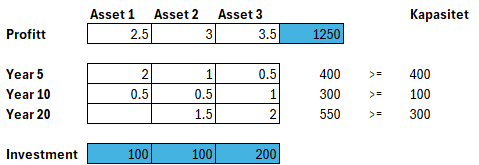
\includegraphics[width=0.8\linewidth]{img/3c.PNG}
    \end{figure}
    
    The table shows returns on investments of \$100 million in asset 1, \$100 million in asset 2 and \$200 million in asset 3. All constraints are satisfied, and the investment of \$400 million would generate \$1.25 billion. Sounds good to me.  
    
    \small\textbf{e)}
    
    \begin{figure}[ht]
        \centering
        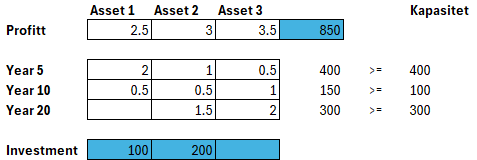
\includegraphics[width=0.8\linewidth]{img/4e.PNG}
    \end{figure}

    Here is the solution found by Excel Solver. The smallest possible investment to satisfy the constraints is \$100 million in asset 1 and \$200 million in asset 2.
    
    \pagebreak\section*{\textbf{Oppgave 4: Distribusjon}}
    \small\textbf{Generell formulering}

    \vspace*{5mm}
    \textit{Indekser:}
    
    i og j: noder i grafen.
    
    \vspace*{5mm}
    \textit{Konstanter og parametre:}
    
    N: antall noder i grafen.
    
    $C_{ij}:$ kostnad per enhet som transporteres mellom node i og j.
    
    $P_i:$ produksjonsmengde hos node i.
    
    $G_{ij}:$ Grense på enheter som kan transporteres mellom node i og j.
    
    \vspace*{5mm}
    \textit{Variabler:}
    
    $x_{ij}:$ antall enheter som transporteres mellom node i og j.
    z: total kostnad til transport av enheter.
    
    \vspace*{5mm}
    \textbf{b)}
    
    min z $= \sum_{i=1}^{N}\sum_{j=1}^{j}x_{ij}C_{ij}$

    \vspace*{5mm}
    s.t.

    $x_{ij} >= 0$, i,j = 1,...,N

    $P_i = \sum_{j=1}^{N}x_{ij} - x_{ji}$, i = 1,...,N

    $x_{ij} <= G_{ij}$

    \begin{align*}
        &\begin{bmatrix}
        \begin{array}{cc|c}
        0 & 0 & 0 \\
        0 & 0 & 0 \\
        0 & 0 & 0
        \end{array}
        \end{bmatrix}
        \end{align*}

    

    \end{document}